\section{Cross-Benchmark Real-Data Validation (SS15)}
\label{sec:ss15}

A single corpus is one verdict. SS15 tests whether the SS10/SS14 pattern
\emph{generalizes} to a second, very different real benchmark---the
conversational tool-use benchmark $\tau$-bench---across two models and two
task domains.

\paragraph{Corpus and provenance.}
We use the publicly released $\tau$-bench trajectory
archive~\cite{taub2024}: Claude-3.5-Sonnet and GPT-4o on the retail and
airline domains, $1{,}980$ episodes in total, each carrying the task reward as
a ground-truth success label. The agent's actions are its \emph{assistant
turns}, mapped to five categories---respond, lookup (read-only tool), write
(state-changing tool), handoff, and think---and the episode absorbs by reward.
Since the MLE and the first-passage KS test depend only on transition counts
and the success-length distribution, we retain per-domain sufficient statistics
and ship the extractor in the artifact.

\paragraph{The asymptotic reliability is accepted---on every domain and model.}
For each of the four model$\times$domain runs
($n = 920$, $400$, $460$, and $200$ episodes) and for the pooled corpus, the
fitted first-order $R_\infty$ recovers the held-out empirical pass rate almost
exactly: the mean absolute error across the four runs is $0.0075$, and the
pooled estimate is $0.595$ versus an observed pass rate of $0.597$
($|{\rm err}|=0.002$). Figure~\ref{fig:calibration} places these estimates
alongside the SWE-agent corpus of \S\ref{sec:ss10}. Panel~(a) plots fitted
$R_\infty$ against the held-out pass rate for all five real corpora: every
point lies on the identity line, and the two hardest ($\tau$-bench airline,
$0.42$--$0.46$) sit on it as tightly as the two easiest, so the estimator is
calibrated over the full competence range, not only where agents succeed
often. Panel~(b) shows the residuals: four corpora and the pooled estimate
fall at or below $0.010$, and the largest---SWE-bench at $0.027$---is an order
of magnitude below the $0.27$ spread in pass rates separating the corpora.
They are also one-signed, $R_\infty$ sitting marginally \emph{below} the
observed rate everywhere, consistent with the conservative exit estimates
censoring induces (\S\ref{sec:robustness}). Calibration therefore holds across
a wide difficulty spread and two underlying models---evidence that the
asymptotic output is trustworthy on real agents, not an artifact of one
corpus. Consequently the
metric-reconciliation and perturbation use cases (which depend only on
$R_\infty$) carry over to $\tau$-bench unchanged.

%% [REDUCTION] tab:ss15 is superseded by Fig.~\ref{fig:calibration}, which plots
%% every pass-rate/$R_\infty$ pair and every residual it listed; the remaining
%% columns ($n$, KS $p$) are quoted inline. Table retained in the artifact.
%% % Auto-generated by SS15_taubench.py
\begin{table}[!t]\centering
\caption{SS15: real-data validation on $\tau$-bench ($1{,}980$ episodes).}
\label{tab:ss15}\small
\begin{tabular}{lrrrrr}
\toprule
domain & $n$ & pass & $R_\infty$ & $|{\rm err}|$ & KS $p$ \\
\midrule
sonnet-retail & 920 & 0.69 & 0.69 & 0.01 & 0.000 \\
sonnet-airline & 400 & 0.46 & 0.45 & 0.01 & 0.001 \\
gpt4o-retail & 460 & 0.60 & 0.60 & 0.01 & 0.000 \\
gpt4o-airline & 200 & 0.42 & 0.41 & 0.01 & 0.000 \\
\textbf{POOLED} & \textbf{1980} & \textbf{0.60} & \textbf{0.59} & \textbf{0.00} & \textbf{0.000} \\
\bottomrule
\end{tabular}
\end{table}


\begin{figure}[!t]
\centering
\begin{tikzpicture}[font=\scriptsize\sffamily, >=Stealth,
  ax/.style={draw=gray!65, line width=0.5pt},
  gr/.style={draw=gray!22, line width=0.3pt},
  pt/.style={circle, draw=blue!70!black, fill=blue!35, line width=0.5pt,
             inner sep=0pt, minimum size=3.0pt},
  ptS/.style={diamond, draw=red!65!black, fill=red!35, line width=0.5pt,
              inner sep=0pt, minimum size=3.6pt},
  ptP/.style={rectangle, draw=black!75, fill=black!25, line width=0.5pt,
              inner sep=0pt, minimum size=3.0pt},
  lab/.style={font=\tiny\sffamily, text=black!70}]
\begin{scope}
  \foreach \v in {0.4,0.5,0.6,0.7}{
    \pgfmathsetmacro\c{(\v-0.38)*9.03}
    \draw[gr] (\c,0) -- (\c,3.25);
    \draw[gr] (0,\c) -- (3.25,\c);
    \node[lab, below=0pt] at (\c,0) {\v};
    \node[lab, left=0pt]  at (0,\c) {\v};
  }
  \draw[ax] (0,0) rectangle (3.25,3.25);
  \draw[gray!65, dashed, line width=0.6pt] (0,0) -- (3.25,3.25);
  \node[lab, rotate=45, anchor=south, text=gray!50!black] at (1.10,1.10) {identity};
  \node[pt]  (a) at (2.84,2.79) {};
  \node[pt]  (b) at (0.74,0.67) {};
  \node[pt]  (c) at (2.02,1.95) {};
  \node[pt]  (d) at (0.36,0.27) {};
  \node[ptP] (p) at (1.96,1.94) {};
  \node[ptS] (s) at (2.74,2.51) {};
  \node[lab, above left=-2pt] at (a.north west) {s-retail};
  \node[lab, right=1pt] at (b.east) {s-airline};
  \node[lab, above left=-2pt] at (c.north west) {g-retail};
  \node[lab, right=1pt] at (d.east) {g-airline};
  \node[lab, right=1pt] at (s.east) {SWE-bench};
  \node[lab, below=1.5pt] at (p.south) {pooled};
  \node[lab] at (1.62,-0.42) {held-out pass rate};
  \node[lab, rotate=90] at (-0.52,1.62) {fitted $R_\infty$};
  \node[font=\scriptsize\sffamily] at (1.62,3.55) {(a) calibration};
\end{scope}
\begin{scope}[shift={(5.08,0)}]
  \foreach \v/\c in {0/0, 0.01/0.85, 0.02/1.70, 0.03/2.55}{
    \draw[gr] (\c,0) -- (\c,3.25);
    \node[lab, below=0pt] at (\c,0) {\v};
  }
  \draw[ax] (0,0) -- (0,3.25);
  \foreach \n/\y/\e/\col in {%
      pooled/0.28/0.002/black!45,
      {s-retail}/0.83/0.005/blue!55,
      {s-airline}/1.38/0.006/blue!55,
      {g-retail}/1.93/0.009/blue!55,
      {g-airline}/2.48/0.010/blue!55,
      {SWE-bench}/3.03/0.027/red!55}{
    \pgfmathsetmacro\w{\e*85}
    \fill[\col] (0,\y-0.15) rectangle (\w,\y+0.15);
    \node[lab, right=1pt] at (\w,\y) {\e};
    \node[lab, left=1.5pt] at (0,\y) {\n};
  }
  \node[lab] at (1.28,-0.42) {$|R_\infty-{}$pass rate$|$};
  \node[font=\scriptsize\sffamily] at (1.28,3.55) {(b) absolute error};
\end{scope}
\end{tikzpicture}
\caption{Fitted $R_\infty$ vs.\ held-out pass rate on five real corpora.}
\label{fig:calibration}
\end{figure}


%% [REDUCTION] fig:ss15 (identity-line scatter) is suppressed for the 12-page body:
%% Table~\ref{tab:ss15} lists every point it plots. Retained in the artifact.
\iffalse
\begin{figure}[!t]
  \centering
  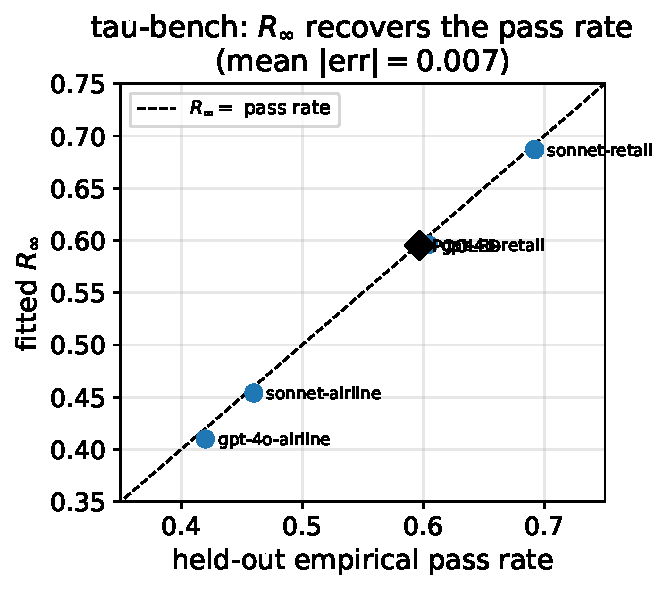
\includegraphics[width=0.62\columnwidth]{../figs/fig_ss15_taubench.pdf}
  \caption{SS15: on real $\tau$-bench traces the fitted $R_\infty$ lies on the
           identity line against the held-out pass rate across both models and
           both domains (mean $|{\rm err}|=0.0075$), replicating the SS14
           SWE-bench finding on a second, conversational benchmark.}
  \label{fig:ss15}
\end{figure}
\fi


\paragraph{The timing behaves exactly as the certificate dictates.}
As on SWE-bench, the success-conditional first-passage KS test rejects the
first-order timing on every domain ($p \le 0.001$ throughout; on sonnet-retail
the empirical median success length is $13$ steps versus a fitted-chain median
of $9$), so the audit
again \emph{withholds} horizon $\mathcal R(d)$ while keeping the accepted
asymptotic and metric outputs. The accept-the-asymptotic /
withhold-the-timing behavior is thus consistent across two independent real
benchmarks, four model$\times$domain corpora, and a wide range of agent
competence.
